\documentclass{article}
\usepackage{amsmath}
\usepackage{amssymb}
\usepackage{bm}
\usepackage[margin=1in]{geometry}
\usepackage{hyperref}
\usepackage{tikz}
\usetikzlibrary{calc, arrows.meta, positioning}

\title{Algorithmic Procedures for Non-Linear Truss Analysis \\ (Bonet \& Wood, Chapter 3)}
\author{}
\date{\today}

\begin{document}

\maketitle

\section*{Step 1: Problem Definition}
Given the initial coordinates $\mathbf{X}$ and material properties (Young's Modulus $E$, Hardening Modulus $H$, Initial Yield Stress $\sigma_{y0}$), find the equilibrium displacements $\mathbf{u}$ such that the internal forces balance the external load $\mathbf{T}_{ext}$.

\section*{Step 2: Global Newton-Raphson Solver}
This is the main loop that finds the equilibrium configuration.

\begin{description}
    \item[Step 2.1: Initialization] 
    Set initial displacements $\mathbf{u} = \mathbf{0}$ and history variables (plastic strain $\varepsilon_p = 0$, accumulated plastic strain $\alpha = 0$).

    \item[Step 2.2: Load Stepping] 
    Increment the external force $\mathbf{T}_{ext}$ or prescribed displacement.

    \item[Step 2.3: Iteration Loop (Newton-Raphson)] 
    Repeat until convergence:
    \begin{description}
        \item[Step 2.3.1: Geometric Update] 
        For each element, calculate the current length $l$ and logarithmic strain $\varepsilon_{n+1}$:
        \begin{align}
            l &= \| \mathbf{x}_2 - \mathbf{x}_1 \| = \| (\mathbf{X}_2 + \mathbf{u}_2) - (\mathbf{X}_1 + \mathbf{u}_1) \| \\
            \varepsilon_{n+1} &= \ln(l/L)
        \end{align}

        \item[Step 2.3.2: Stress Update] 
        Execute the \textbf{Material Point Algorithm} (see Step 3) for each element to obtain the Kirchhoff stress $\tau_{n+1}$ and the algorithmic tangent modulus $E_{alg}$.

        \item[Step 2.3.3: Assembly] 
        Compute element internal force $\mathbf{f}_{int}$ and stiffness $\mathbf{k}_{tan}$ (see Step 4) and assemble them into the global vector $\mathbf{T}_{int}$ and matrix $\mathbf{K}$.

        \item[Step 2.3.4: Residual Calculation] 
        Compute the residual force vector:
        \begin{equation}
            \mathbf{R} = \mathbf{T}_{ext} - \mathbf{T}_{int}
        \end{equation}

        \item[Step 2.3.5: Convergence Check] 
        If $\|\mathbf{R}\| < \text{tolerance}$, update history variables ($\varepsilon_{p,n} \leftarrow \varepsilon_{p,n+1}$) and proceed to the next Load Step (Step 2.2).

        \item[Step 2.3.6: Linear Solve] 
        Solve for the displacement increment $\delta \mathbf{u}$:
        \begin{equation}
            \mathbf{K} \delta \mathbf{u} = \mathbf{R}
        \end{equation}

        \item[Step 2.3.7: Update Configuration] 
        Update total displacements:
        \begin{equation}
            \mathbf{u} \leftarrow \mathbf{u} + \delta \mathbf{u}
        \end{equation}
    \end{description}
\end{description}

\section*{Step 3: Material Point Algorithm (Return Mapping)}
This algorithm is executed at the integration point level (for trusses, one per element) to update stress and plastic variables.

\begin{description}
    \item[Step 3.1: Elastic Predictor] 
    Assume the step is purely elastic. Use history variables from the previous converged step $n$.
    \begin{align}
        \tau^{trial} &= E (\varepsilon_{n+1} - \varepsilon_{p,n}) \\
        \Phi^{trial} &= |\tau^{trial}| - (\sigma_{y0} + H \alpha_n)
    \end{align}

    \item[Step 3.2: Plastic Corrector Check] 
    Check the yield function $\Phi^{trial}$:
    
    \textbf{Case A: Elastic Step} ($\Phi^{trial} \le 0$)
    \begin{equation}
        \tau_{n+1} = \tau^{trial}, \quad E_{alg} = E
    \end{equation}
    Update trial variables: $\varepsilon_{p,n+1} = \varepsilon_{p,n}, \quad \alpha_{n+1} = \alpha_n$.

    \textbf{Case B: Plastic Step} ($\Phi^{trial} > 0$)
    \begin{enumerate}
        \item Calculate plastic multiplier increment:
        \begin{equation}
            \Delta \gamma = \frac{\Phi^{trial}}{E + H}
        \end{equation}
        \item Correct the stress (Return to yield surface):
        \begin{equation}
            \tau_{n+1} = \tau^{trial} - E \Delta \gamma \, \text{sign}(\tau^{trial})
        \end{equation}
        \item Update plastic variables:
        \begin{align}
            \varepsilon_{p,n+1} &= \varepsilon_{p,n} + \Delta \gamma \, \text{sign}(\tau^{trial}) \\
            \alpha_{n+1} &= \alpha_n + \Delta \gamma
        \end{align}
        \item Compute Consistent Tangent Modulus:
        \begin{equation}
            E_{alg} = \frac{EH}{E + H}
        \end{equation}
    \end{enumerate}
\end{description}

\section*{Step 4: Finite Element Formulation (Derivation \& Proof)}

This section provides the derivation of the internal force vector and tangent stiffness matrix using the Principle of Virtual Work and index notation.

\subsection*{Step 4.1: Kinematics and Definitions}

Consider a truss element with two nodes, 1 and 2.
\begin{itemize}
    \item $\mathbf{X}_a$: Reference coordinates of node $a$ ($a=1,2$).
    \item $\mathbf{x}_a = \mathbf{X}_a + \mathbf{u}_a$: Current coordinates of node $a$.
    \item $L = \|\mathbf{X}_2 - \mathbf{X}_1\|$: Initial length.
    \item $l = \|\mathbf{x}_2 - \mathbf{x}_1\|$: Current length.
    \item $\mathbf{n} = \frac{\mathbf{x}_2 - \mathbf{x}_1}{l}$: Current unit vector.
\end{itemize}

\begin{center}
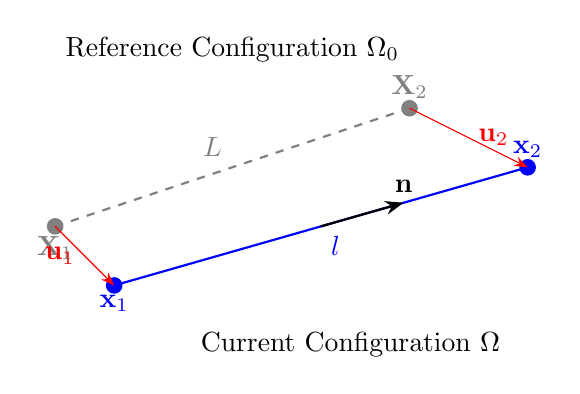
\begin{tikzpicture}[scale=1.5, >=Stealth]
    % Reference Configuration
    \coordinate (X1) at (0,0);
    \coordinate (X2) at (3,1);
    
    \draw[dashed, gray, thick] (X1) -- (X2) node[midway, above left] {$L$};
    \fill[gray] (X1) circle (2pt) node[below] {$\mathbf{X}_1$};
    \fill[gray] (X2) circle (2pt) node[above] {$\mathbf{X}_2$};
    
    % Current Configuration
    \coordinate (x1) at (0.5, -0.5);
    \coordinate (x2) at (4, 0.5);
    
    \draw[thick, blue] (x1) -- (x2) node[midway, below right] {$l$};
    \fill[blue] (x1) circle (2pt) node[below] {$\mathbf{x}_1$};
    \fill[blue] (x2) circle (2pt) node[above] {$\mathbf{x}_2$};
    
    % Displacement Vectors
    \draw[->, red] (X1) -- (x1) node[midway, left] {$\mathbf{u}_1$};
    \draw[->, red] (X2) -- (x2) node[midway, right] {$\mathbf{u}_2$};
    
    % Unit Vector
    \draw[->, thick, black] ($(x1)!0.5!(x2)$) -- ($(x1)!0.7!(x2)$) node[above] {$\mathbf{n}$};
    
    \node at (1.5, 1.5) {Reference Configuration $\Omega_0$};
    \node at (2.5, -1) {Current Configuration $\Omega$};
\end{tikzpicture}
\end{center}

\subsection*{Step 4.2: Derivation of Internal Force Vector}

The internal virtual work $\delta W_{int}$ is defined as the integral of the stress work over the reference volume $V$. For a truss element with constant cross-section $A$ and length $L$, assuming constant stress $\tau$ (Kirchhoff stress) and logarithmic strain $\varepsilon$:
\begin{equation}
    \delta W_{int} = \int_{V} \tau \delta \varepsilon \, dV = V \tau \delta \varepsilon
\end{equation}
The logarithmic strain is $\varepsilon = \ln(l/L)$. Its variation is:
\begin{equation}
    \delta \varepsilon = \delta (\ln l - \ln L) = \frac{1}{l} \delta l
\end{equation}
The current length squared is $l^2 = (\mathbf{x}_2 - \mathbf{x}_1) \cdot (\mathbf{x}_2 - \mathbf{x}_1)$. Taking the variation:
\begin{align}
    2 l \delta l &= 2 (\mathbf{x}_2 - \mathbf{x}_1) \cdot (\delta \mathbf{x}_2 - \delta \mathbf{x}_1) \\
    l \delta l &= (\mathbf{x}_2 - \mathbf{x}_1) \cdot (\delta \mathbf{u}_2 - \delta \mathbf{u}_1) \\
    \delta l &= \frac{\mathbf{x}_2 - \mathbf{x}_1}{l} \cdot (\delta \mathbf{u}_2 - \delta \mathbf{u}_1) = \mathbf{n} \cdot (\delta \mathbf{u}_2 - \delta \mathbf{u}_1)
\end{align}
Substituting $\delta \varepsilon = \frac{1}{l} \mathbf{n} \cdot (\delta \mathbf{u}_2 - \delta \mathbf{u}_1)$ into the virtual work equation:
\begin{equation}
    \delta W_{int} = V \tau \left( \frac{1}{l} \mathbf{n} \cdot (\delta \mathbf{u}_2 - \delta \mathbf{u}_1) \right) = \frac{V \tau}{l} \mathbf{n} \cdot \delta \mathbf{u}_2 - \frac{V \tau}{l} \mathbf{n} \cdot \delta \mathbf{u}_1
\end{equation}
The internal force vector $\mathbf{f}_{int}$ is defined such that $\delta W_{int} = \mathbf{f}_{int} \cdot \delta \mathbf{u}$. Thus, the nodal forces are:
\begin{equation}
    \mathbf{f}_1 = -\frac{V \tau}{l} \mathbf{n}, \quad \mathbf{f}_2 = \frac{V \tau}{l} \mathbf{n}
\end{equation}
In matrix form:
\begin{equation}
    \mathbf{f}_{int} = \frac{V \tau}{l} \begin{bmatrix} -\mathbf{n} \\ \mathbf{n} \end{bmatrix}
\end{equation}

\subsection*{Step 4.3: Derivation of Tangent Stiffness Matrix}

The tangent stiffness matrix $\mathbf{k}$ relates the change in force to the change in displacement: $d\mathbf{f}_{int} = \mathbf{k} d\mathbf{u}$.
We differentiate $\mathbf{f}_2 = F \mathbf{n}$ where $F = \frac{V \tau}{l}$.
\begin{equation}
    d\mathbf{f}_2 = dF \mathbf{n} + F d\mathbf{n}
\end{equation}

\subsubsection*{Step 4.3.1: Material Stiffness (Term 1)}
The term $dF \mathbf{n}$ represents the change in force magnitude due to material deformation.
\begin{equation}
    dF = d\left( \frac{V \tau}{l} \right) = V \left( \frac{d\tau}{l} - \frac{\tau dl}{l^2} \right)
\end{equation}
Using the constitutive relation $d\tau = E_{alg} d\varepsilon = E_{alg} \frac{dl}{l}$:
\begin{equation}
    dF = V \left( \frac{E_{alg} dl}{l^2} - \frac{\tau dl}{l^2} \right) = \frac{V}{l^2} (E_{alg} - \tau) dl
\end{equation}
Assuming small strains or defining the algorithmic modulus such that it dominates, we approximate $E_{alg} - \tau \approx E_{alg}$ (or define the material stiffness based on the primary constitutive term). Thus:
\begin{equation}
    dF \approx \frac{V E_{alg}}{l^2} dl = \frac{V E_{alg}}{l^2} (\mathbf{n} \cdot d\mathbf{u}_{21})
\end{equation}
The material stiffness contribution to the force vector is:
\begin{equation}
    d\mathbf{f}_{2, mat} = \left[ \frac{V E_{alg}}{l^2} (\mathbf{n} \cdot d\mathbf{u}_{21}) \right] \mathbf{n} = \frac{V E_{alg}}{l^2} (\mathbf{n} \otimes \mathbf{n}) d\mathbf{u}_{21}
\end{equation}
This yields the material stiffness matrix block:
\begin{equation}
    \mathbf{k}_{mat} = \frac{V E_{alg}}{l^2} (\mathbf{n} \otimes \mathbf{n})
\end{equation}

\subsubsection*{Step 4.3.2: Geometric Stiffness (Term 2)}
The term $F d\mathbf{n}$ represents the change in force direction due to rotation.
We need the variation of the unit vector $\mathbf{n} = \mathbf{x}_{21} / l$. Using index notation:
\begin{align}
    d n_i &= d\left( \frac{x_i}{l} \right) = \frac{dx_i}{l} - \frac{x_i dl}{l^2} \\
    &= \frac{du_i}{l} - \frac{x_i}{l^2} (n_k du_k) \\
    &= \frac{1}{l} (\delta_{ik} - n_i n_k) du_k
\end{align}
In vector notation:
\begin{equation}
    d\mathbf{n} = \frac{1}{l} (\mathbf{I} - \mathbf{n} \otimes \mathbf{n}) d\mathbf{u}_{21}
\end{equation}
Substituting this into the force variation term:
\begin{equation}
    d\mathbf{f}_{2, geo} = F d\mathbf{n} = \frac{V \tau}{l} \left[ \frac{1}{l} (\mathbf{I} - \mathbf{n} \otimes \mathbf{n}) d\mathbf{u}_{21} \right]
\end{equation}
This yields the geometric stiffness matrix block:
\begin{equation}
    \mathbf{k}_{geo} = \frac{V \tau}{l^2} (\mathbf{I} - \mathbf{n} \otimes \mathbf{n})
\end{equation}

\subsubsection*{Step 4.3.3: Total Element Stiffness}
Combining the material and geometric parts for the full element (relating $\begin{bmatrix} d\mathbf{f}_1 \\ d\mathbf{f}_2 \end{bmatrix}$ to $\begin{bmatrix} d\mathbf{u}_1 \\ d\mathbf{u}_2 \end{bmatrix}$):
\begin{equation}
    \mathbf{K} = \left( \mathbf{k}_{mat} + \mathbf{k}_{geo} \right) \begin{bmatrix} 1 & -1 \\ -1 & 1 \end{bmatrix}
\end{equation}
where the block matrices are:
\begin{align}
    \mathbf{k}_{mat} &= \frac{V E_{alg}}{l^2} (\mathbf{n} \otimes \mathbf{n}) \\
    \mathbf{k}_{geo} &= \frac{V \tau}{l^2} (\mathbf{I} - \mathbf{n} \otimes \mathbf{n})
\end{align}

\end{document}
